\section{Auswertung}
\label{sec:Auswertung}

\subsection{Die Aktivit"at der Americum-Quelle}
  Die Aktivit"at/Z"ahlrate $Z_{Quelle}$ der $^{241}\text{Am}$-Quelle wird gegeben druch
  \begin{equation}
    \frac{4\pi(\SI{0,041}{\meter}+\SI{0,039}{\meter}+\SI{0.017}{\meter})^2}{3F}Z_{gemessen}
  \end{equation}
  ,weil davon ausgegangen wird, dass die Quelle homogen in alle Raumrichtungen strahlt.
  Mit $Z_{gemessen}=\SI{13,5}{\becquerel}$ ergibt sich:
  \begin{equation}
    Z_{Quelle} = \SI{274}{\kilo \becquerel} \; .
  \end{equation}

  Der theoretisch zu erwartende Wert kann mithilfe des klassischen Zerfallsgesetzes berechnet werden:
  \begin{equation}
    Z_{Quelle} = Z_0\text{e}^{\frac{\ln(2)t}{\tau}} \approx \SI{318}{\kilo \becquerel}
  \end{equation}
  Dabei ist $\tau=432,2$ Jahre die Halbwertszeit und $Z_0=\SI{330}{\kilo \becquerel}$ \cite{Anleitung} die urspr"ungliche Aktivit"at.


\subsection{\texorpdfstring{Bestimmung der Foliendicke einer Goldfolie durch Energieverlustmessung der $\alpha$-Teilchen}{Bestimmung der Foliendicke einer Goldfolie durch Energieverlustmessung der alpha-Teilchen}}
Zur Bestimmung der Foliendicke wurde eine Energieverlustmessung durchgeführt.
Die Messwerte sind in Tabelle 2 und 3 aufgelistet. 
\begin{table}[H] 
	\centering
	\begin{tabular}{c|c}

		Druck  [mbar]& Pulshöhe [mV] \\ 
		\hline 
0,059	&1020 \\
20	&960 \\
30	&900\\
40	&860\\
50	&840\\
60	&820\\
70	&720\\
80	&740\\
90	&730\\
100	&680\\
110	&640\\
120	&620\\
130	&610\\
140	&600\\	
		
	\end{tabular} 
	\caption{Messwerte für die Energieverlustmessung mit Folie } 
\end{table}  

\begin{table}[H] 
	\centering
	\begin{tabular}{c|c}

	Druck[mbar] & Pulshöhe  [V] \\ 
		\hline 
0,07	& 1480\\
40	& 1300\\
80	& 1160\\
120	& 1040\\
140	& 940\\
	
	\end{tabular} 
	\caption{Messwerte für die Energieverlustmessung ohne Folie } 
\end{table} 

Die Werte für die Pulshöhe werden gegen den Druck aufgetragen. \\ Mittels linearer Regression ergibt sich folgender Graph:   
\begin{figure}[h]
	\centering
	\includegraphics[width=12cm,height=8cm]{auswertung/v16_plot1.pdf}
	\caption{Energieverlustmessung mit und ohne Goldfolie}
	\label{img:grafik-dummy}
\end{figure}
\newpage 
Aus der Ausgleichsrechnung ergeben sich für die Parameter m und b der Funktion $f(x)=m\cdot x+b$ für die Messung mit und ohne eingesetzter Folie folgende Werte: 
\begin{align*}
m_{ohne}= -3,71 \pm 0,1602 \; \frac{1}{\text{mbar}}
\\
m_{mit}= -3,09 \pm 0,1578 \; \frac{1}{\text{mbar}}
\\
\\
b_{ohne}= 1466,4 \pm 14,68 \; \text{mV}
\\
b_{mit}= 996,82 \pm  13,43 \; \text{mV}
\end{align*}
Die Differenz dieser beiden Geraden entspricht dem Energieverlust durch die Folie. Durch die Subtraktion der Achsenabschnitte wird zunächst die Differenz der Impulshöhen bestimmt: 
\begin{align}
\Delta I= b_{ohne}-b_{mit}= 469,58 \pm 28,11 \; \text{mV}
\end{align} 
Aus dem Termschema in Abbildung 2 lässt sich für die Energie des $\alpha$-Teilchens der Wert E=5.486 MeV ablesen. Im Folgenden wird angenommen, dass das die Energie ist, die bei der Messung ohne Folie am Detektor detektiert wird. Unter dieser Annahme lässt sich der Energieverlust mit der Differenz der Impulshöhen (4) berechnen zu: 
\begin{align*}
\Delta E= 1,7568 \pm 0,10\;  \text{MeV}  
\end{align*} 

Mit dem Energieverlust lässt sich durch Umstellen der Bethe-Bloch-Gleichung (1) und Einsetzen der folgenden materialabhängigen Parameter die Dicke der Folie dx bestimmen.  
Die Masse des $\alpha$-Teilchens lässt sich über $m=A \cdot u$ bestimmen. Dabei ist A die elementspezifische Massenzahl und u die atomare Masseneinheit. Für ein $\alpha$-Teilchen gilt A=4 sodass sich für die Masse folgender Wert ergibt: 

\begin{align*}
m_{\alpha}= 6.64 \cdot 10^{-27} \text{kg} 
\end{align*} 
damit lässt sich die Geschwindigkeit mit \begin{align*}
v_{\alpha}= \sqrt{\frac{2\cdot E_{\alpha}}{m_{\alpha}}} 
\end{align*} 
bestimmen:
\begin{align*}
v_{\alpha}=16.27 \cdot 10^{6} \frac{\text{m}}{\text{s}}
\end{align*} 

Die Anzahl der Teilchen pro Volumeneinheit N lässt sich über \begin{align}
N= \frac{\rho}{m} 
\end{align} bestimmen. Für die Dichte des Targetmaterials $\rho$ wird 19320 $\frac{\text{kg}}{\text{m}^3}$ $[1]$ eingesetzt. Die Masse wird wieder mittels des Produktes aus Massenzahl und atomarer Masseneinheit bestimmt. \\ Daraus ergibt sich für die Masse von Gold (A=197 $[5]$): $m_{Gold}=1.31 \cdot 10^{-25}$ kg und damit folgende  Anzahl der Teilchen pro $\text{m}^3$: 
 \begin{align*}
 5.91 \cdot 10^{28} \frac{1}{\text{m}^3}
 \end{align*} 
 Aus den berechneten Werten und der Ionisationsenergie von Gold $I=9.225 \frac{\text{eV}}{\text{atom}} \; [5]$ und den Ordnungzahlen Z$_{\alpha}$=2 und Z$_{Gold}$=79 ergibt sich folgender Wert:
 \begin{align*}
 dx= ( \pm ) \; \mu \text{m}
 \end{align*}

\subsection{Vermessung des Rutherford-Streugesetzes}
  Die gemessenen Z"ahlraten $Z(\theta)$ und zugeh"origen Streuwinkel $\theta$ so wie der jeweils nach Formel (\ref{querschnitt}) berechnete differentielle Wirkungsquerschnitt $\text{d}\sigma/\text{d}\Omega(\theta)$ sind in Tabelle (\ref{tab:ruther}) dargestellt.
  Dabei sind
  \begin{align*}
    F &= \SI{20e-6}{\meter \squared} \\
  \end{align*}


  \begin{table}
  \centering
  \begin{tabular}{c|c|c}

  Streuwinkel $\theta$ /Grad	&	Z"ahlrate $Z(\theta)/\frac{1}{\SI{60}{\second}}$	& $\frac{\text{d}\sigma}{\text{d}\Omega(\theta)}/\si{\meter \squared}$	 \\

  \toprule
 	0	   & 776 & 4.47e-21 \\
 	0,2	 & 662 & 3.82e-21 \\
 	0,4	 & 669 & 3.86e-21 \\
 	0,6	 & 583 & 3.36e-21 \\
  0,8  & 586 & 3.38e-21 \\
  1    & 612 & 3.53e-21 \\
  1,2  & 630 & 3.63e-21 \\
  1,4  & 635 & 3.66e-21 \\
  1,6  & 604 & 3.48e-21 \\
  1,8  & 642 & 3.70e-21 \\
  2    & 633 & 3.70e-21 \\
  2,2  & 615 & 3.55e-21 \\
  2,4  & 549 & 3.42e-21 \\
  2,6  & 621 & 3.58e-21 \\
  2,8  & 616 & 3.55e-21 \\
  3    & 634 & 3.66e-21 \\
  7    & 424 & 2.45e-21 \\
  10   & 260 & 1.50e-21 \\
  15   & 85  & 4.99e-22 \\
  20   & 26  & 1.52e-22 \\
 %\midrule

  %\multicolumn{2}{c}{$\overline{n}$} & \multicolumn{2}{c} {1,56 $\pm$ 0,02} \\
 \bottomrule
  \end{tabular}
  \caption{Streuwinkel und zugeh"orige Z"ahlrate so wie differentieller Wirkungsquerschnitt f"ur die $\SI{2}{\micro \meter}$-Goldfolie.}
  \label{tab:ruther}
  \end{table}


  Die experimentellen Werte ($\theta,\frac{\text{d}\sigma}{\text{d}\Omega(\theta)}$) sind zusammen mit der Theoriekurve nach (\ref{ruther}) in Abb. (\ref{plot:ruther}) aufgetragen.

  \begin{figure}
    \centering
    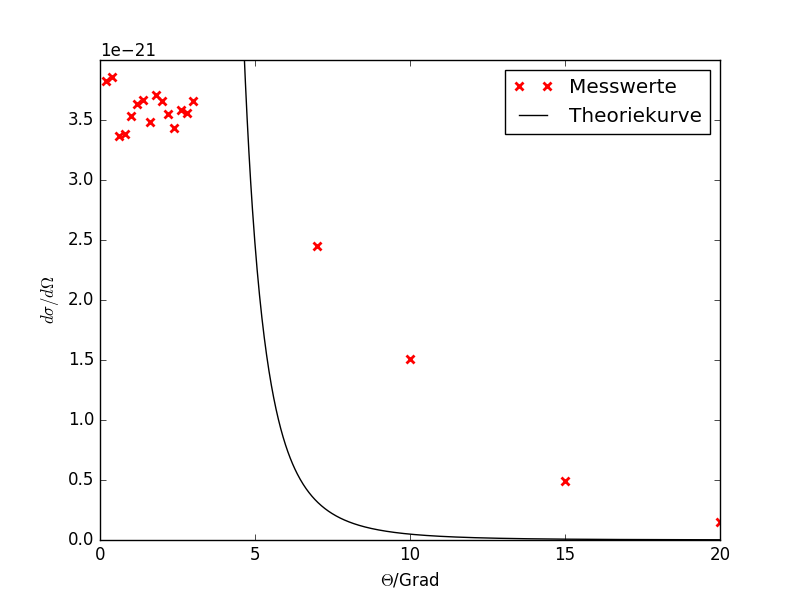
\includegraphics[width=15cm]{skripte/ruther.png}
    \caption{Messwerte und Theoriekurve f"ur das Rutherford-Streugesetz bei der $\SI{2}{\micro \meter}$-Goldfolie.}
    \label{plot:ruther}
  \end{figure}

  Wie zu erkennen ist, zeigen die Messwerte neben dem insgesamt abfallendem Trend keine gute "Ubereinstimmung mit der Theoriekurve.

  \newpage



  \subsection{Nachweis von Mehrfachstreuungen und und $Z$-Abh"angigkeit der Rutherford-Streuformel}



Die Messwerte für die Folien aus verschiedenen Materialien sind in Tabelle 7 aufgelistet. Außerdem sind die zur Berechnung des Wirkungsquerschnittes benötigten Stoffeigenschaften ebenfalls in Tabelle 7 zu finden. 

\begin{table}[H] 
\centering
\begin{tabular}{c|c c c c c c c}

	Folienmaterial &Dichte $\rho [\frac{kg}{m^3}]$& Z & A & N [$\cdot 10^{28} \frac{1}{m^3}$]& Zeit t [s]& Zählrate n & n/t [s$^{-1}$]  \\ 
	\hline 
	Aluminium (3 $\mu$m) &2,7 $\cdot 10^{4}$& 13 & 27& 6,022 & 120  & 619 & 5,15  \\ 

	Bismut (1 $\mu$m)& 9,78 $\cdot 10^{4}$  & 83 & 209& 2,818 & 120 & 705 & 5,87 \\ 

	Gold (2 $\mu$m) & 1,93   $\cdot 10^{4}$ & 79 & 197 & 5.910 & 120 & 121 & 1,008 \\ 

\end{tabular} 
	\caption{Messwerte für Folien aus unterschiedlichem Material} 
\end{table}
 
 Die aus diesen Werten mittels der Formeln (2) und (7) berechneten Wirkungsquerschnitte sind in Tabelle 8 aufgelistet:
 
 \begin{table}[H] 
 	\centering
 	\begin{tabular}{c|c c }
 		
 		Folienmaterial & $\frac{d\sigma}{d\Omega}_{Theorie}[ 10^{-24} \frac{1}{m}]$& $\frac{d\sigma}{d\Omega}_{Gemessen}[ 10^{-21} \frac{1}{m}]$ \\ 
 		\hline 
 		
 		Aluminium & 0.050 & 8.536 $\pm$ 5.413 \\ 
 		
 		Bismut & 2.056 & 3.567 $\pm$ 8.503   \\
 		
 		Gold & 1.863 & 8.215 $\pm$ 6.468 \\ 
 		
 	\end{tabular} 
 	\caption{Wirkungsquerschnitte für Folien aus verschiedenem Material} 
 \end{table}
Um die Z-Abhängigkeit zu untersuchen, wird in Abbildung 5 $\frac{n}{N\cdot dx}$ gegen die Ordnungszahl Z aufgetragen: 
\begin{figure}[H]
	\centering
	\includegraphics[width=12cm,height=8cm]{Z.pdf}
	\caption{Z-Abhängigkeit}
	\label{img:grafik-dummy}
\end{figure}
